\documentclass[11pt]{scrartcl}
\usepackage{graphicx}
\graphicspath{{./}}
\usepackage[sexy]{evan}
\usepackage[normalem]{ulem}
\usepackage{hyperref}
\usepackage{mathtools}
\hypersetup{
    colorlinks=true,
    linkcolor=blue,
    filecolor=magenta,      
    urlcolor=cyan,
    pdfpagemode=FullScreen,
    }

\renewcommand{\dangle}{\measuredangle}

\renewcommand{\baselinestretch}{1.5}

\addtolength{\oddsidemargin}{-0.4in}
\addtolength{\evensidemargin}{-0.4in}
\addtolength{\textwidth}{0.8in}
% \addtolength{\topmargin}{-0.2in}
% \addtolength{\textheight}{1in} 


\setlength{\parindent}{0pt}

\usepackage{pgfplots}
\pgfplotsset{compat=1.15}
\usepackage{mathrsfs}
\usetikzlibrary{arrows}

\usepackage[most]{tcolorbox}

\title{Soal Campur 2}
\author{Compiled by Azzam}

\date{Jumat, 22 Maret 2024}
\begin{document}
\maketitle
\textbf{Waktu: 180 menit}

\begin{enumerate}
    \item Notasikan $\tau(n)$ sebagai banyak faktor positif dari $n$. Nilai dari
        $$1 \times (-1)^{\tau(1)} + 2 \times (-1)^{\tau(2)} + 3 \times (-1)^{\tau(3)} + \ldots + 200 \times (-1)^{\tau(200)}$$
        adalah...
    \item Diberikan persegi panjang $ABCD$ dengan $AB = 3$ dan $BC = 6$. $M$ merupakan titik pada $BC$ sedemikian hingga $\angle AMB = \angle AMD$. Besar sudut $\angle BAM$ adalah...
    \item Diketahui $ab + cd = 1$ dan $abc = d + 3$. Nilai dari $a^2b^2 + d^2$ jika diketahui $|c| = 1$ adalah...
    \item Banyak bilangan asli kurang dari 1000 yang memiliki jumlah digit habis dibagi 8 dan bilangan tersebut habis dibagi 3 adalah...
    \item Diketahui bahwa $3^{27} + 1$ memiliki 2 faktor prima lebih dari 100. Jumlah dari ketiga bilangan tersebut adalah...
    \item Analit FC, Bary Saint-Germain, Invers Milan, Har-Münich, Real Complex, Atlético Euclid, dan Trigonspor adalah tujuh tim yang mengikuti Liga Sepakbola Geo. Setiap tim bertanding melawan tim lain sebanyak satu kali. Kemenangan mendapat 3 poin, seri mendapat 1 poin, dan kekalahan mendapat 0 poin. Diketahui pada akhir liga, jumlah poin seluruh tim adalah 48. Trigonspor menjadi peringkat 1 dengan selisih poin 1 dengan tim peringkat 2. Trigonspor juga tak pernah mencatatkan pertandingan seri. Hasil kali poin seluruh tim adalah...
    \item Delapan buah persegi identik dengan panjang sisi 5 disusun di dalam sebuah persegi besar seperti pada gambar di bawah.\\
            \begin{figure}[h]
                \centering
                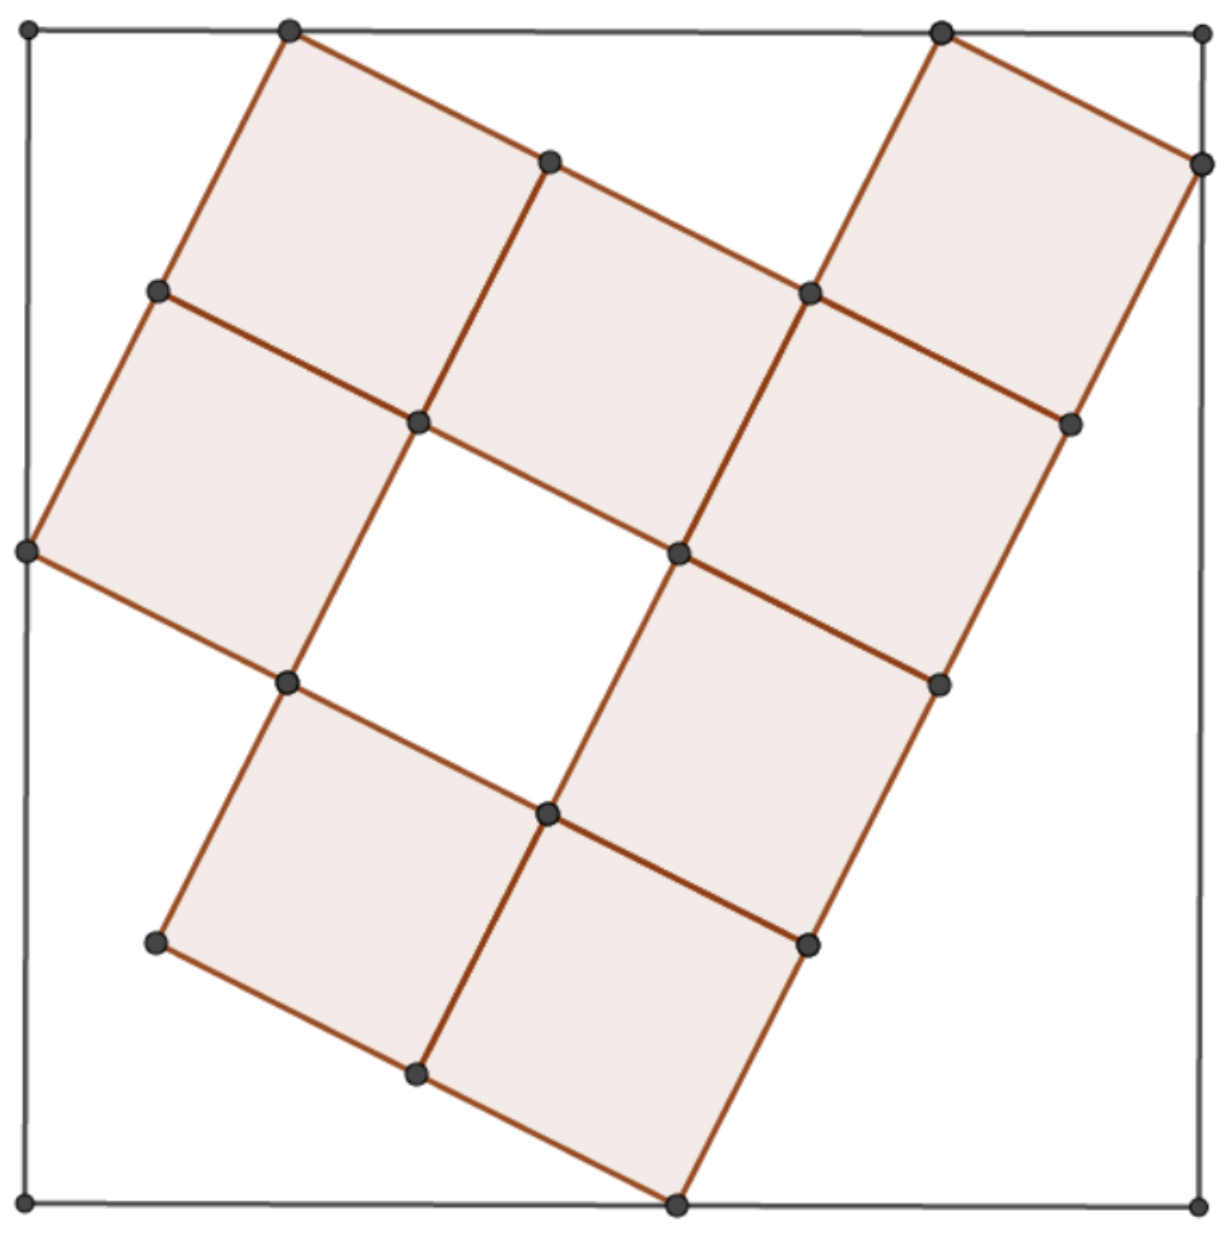
\includegraphics[scale=0.3]{Test For Pelatihan/EDUOS 22-23 Maret 2024/geom.png}
            \end{figure}
        Luas persegi besar adalah...
    \item Misal $a$, $b$, $c$ merupakan tiga bilangan real tak nol yang memenuhi persamaan
        $$bc + \frac{1}{a} = ca + \frac{2}{b} = ab + \frac{7}{c} = \frac{1}{a + b + c}$$
        Nilai dari $a^3 + 8b^3 + c^3$ adalah...
    \item Sebut suatu bilangan asli $k$ kjokkenmoddinger jika untuk setiap bilangan asli $n$, $\text{FPB}(4n+1, kn+1) = 1$. Jumlah seluruh bilangan kjokkenmoddinger yang lebih kecil dari 200 adalah...
    \item Diberikan segitiga $ABC$ lancip. $H$ adalah proyeksi $C$ terhadap $AB$. $M$ dan $N$ secara berturut-turut adalah proyeksi $H$ ke $BC$ dan $CA$. Diketahui pula bahwa titik pusat lingkaran luar segitiga $ABC$ terletak di garis $MN$ dan panjang jari-jari lingkaran luar tersebut adalah 2. Jika panjang $CH$ adalah $n$, maka nilai dari $n^2$ adalah...
\end{enumerate}

\begin{enumerate}[resume]
    \item Banyak pasangan bilangan real $(x, y)$ sedemikian hingga $x^2 + y^2 = \frac{25}{2}$ dan $6x + y^2 = 15 + x^2$ adalah...
    \item Sebuah bilangan asli $n$ disebut sebagai primakasih jika setiap sub-bilangan dua digit dari $n$ merupakan bilangan prima. Contohnya, 3719 termasuk bilangan primakasih karena 37, 71, dan 19 adalah bilangan prima. Banyak bilangan primakasih 4 digit adalah...
    \item Misalkan $p$ dan $q$ adalah dua bilangan prima sedemikian hingga $p$ merupakan faktor dari $7q - 1$ dan $q$ merupakan faktor dari $7p - 1$. Jumlah dari seluruh nilai $p$ yang mungkin adalah...
    \item Diberikan persegi $ABCD$. $P$ adalah titik yang terletak di dalam segitiga $ABC$ sedemikian hingga $\angle CAP = \angle BCP = \frac{15^\circ}{2}$. Titik $Q$ dipilih sedemikian hingga $PC$ sejajar dengan $AQ$, $AP = CQ$, dan $AP$ tidak sejajar dengan $CQ$. Jika $N$ adalah titik tengah $PQ$, maka besar sudut $\angle CAN$ adalah...
    \item Misal $a$, $b$, $c$ adalah tiga buah bilangan real positif yang memenuhi $a + 2b + 3c = 36$. Jika nilai minimum dari
        $$(a^3 + 35)(b^3 + 224)(c^3 + 243)$$
        adalah $N$, maka banyak faktor positif dari $N$ adalah...
\end{enumerate}

\begin{enumerate}[resume]
    \item Untuk tiap bilangan asli $n$, definisikan $a_n$ sebagai banyak bilangan asli $n$ digit yang digitnya hanya menggunakan angka 1 dan 2, serta tidak ada dua angka 2 yang terletak persis bersebelahan. Nilai dari $a_{15}$ adalah...
    \item Jumlah seluruh bilangan bulat prima $p$ sedemikian hingga $1 + p + p^2 + p^3 + p^4$ merupakan bilangan kuadrat adalah...
    \item Diberikan segitiga $ABC$ dengan $AB = 3$, $BC = 4$, dan $CA = 5$. $D$ merupakan proyeksi $B$ terhadap $AC$. $O$ merupakan titik pusat lingkaran luar segitiga $ABC$. $E$ merupakan perpotongan $BD$ dengan lingkaran luar segitiga $ABC$. $M$, $N$, dan $P$ berturut-turut adalah titik tengah $AE$, $DO$, dan $BC$. $Q$ merupakan proyeksi $N$ terhadap $AB$. Nilai dari $\frac{NQ}{MP}$ adalah...
    \item Faiq dan Fauzi sedang bermain dengan papan catur berukuran $5 \times 5$. Dimulai dari Faiq, secara bergantian mereka berdua menuliskan angka ke dalam petak catur. Faiq menuliskan angka 1 dan Fauzi menuliskan angka 0, sampai seluruh petak catur penuh. Untuk setiap petak $3 \times 3$, jumlah dari kesembilan angkanya dihitung. Misalkan $A$ adalah nilai terbesar dari jumlah-jumlah tersebut. Nilai maksimal dari $A$ yang mungkin didapat jika Fauzi bermain dengan semangat meminimalkan nilai $A$ adalah...
    \item Misalkan suatu barisan bilangan $F_n$ memenuhi $F_0 = 0$, $F_1 = 1$, dan $F_n = F_{n-1} + F_{n-2}$ untuk $n$ bilangan asli lebih besar dari 1. Diketahui bahwa ketika nilai $n$ semakin besar, nilai $\frac{F_n}{F_{n-1}}$ semakin mendekati $\frac{1 + \sqrt{5}}{2}$. Misalkan
        $$N = \sum_{n=0}^\infty \frac{1}{F_{2^n}}$$
        Nilai dari $4N^2 - 14N + 40$ adalah...
\end{enumerate}

\end{document}